\documentclass[../main.tex]{subfiles}
\graphicspath{{\subfix{../media/}}}


\begin{document}
	
	\begin{figure}[h]
	    \centering
	    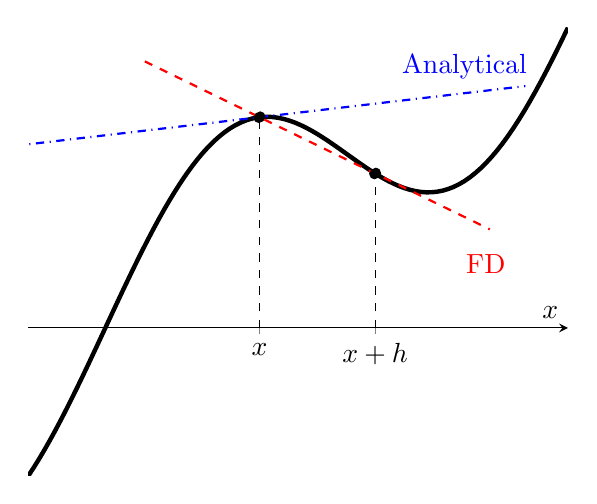
\begin{tikzpicture}
	        % Points stencil
	        \def\pointx{2}
	        \def\pointh{3.5}
	        
	        \begin{axis}[
	            xlabel = $x$,
	            ylabel = $f(x)$,
	            hide y axis,
	            xtick = {\pointx, \pointh},
	            xticklabels = {$x$, $x+h$},
	            axis lines = middle,  
	            declare function={
	                func(\x) = 2*sin(deg(\x)) + \x;
	            }
	        ]
	            
	            % Function
	            \addplot[ultra thick, domain=-1:6, samples=100, label={center:$f(x)$}] {func(x)};
	            \addplot[samples at={\pointx, \pointh}, mark=*, ycomb, dashed] {func(x)};
	            
	            % Nodes for x values
	            \node[name=nodeA] at (axis cs: \pointx, {func(\pointx)}) {};
	            \node[name=nodeC] at (axis cs: \pointx+0.01, {func(\pointx+0.01)}) {};
	            \node[name=nodeB] at (axis cs: \pointh, {func(\pointh)}) {};
	            
	            % Derivatives approx. and analytical
	            \draw[red, dashed, thick, shorten >= -50pt, shorten <=-50pt] (nodeA) -- (nodeB) node[above, align= center, xshift=40pt, yshift=-40pt] {FD};
	            \draw[dash dot, blue, thick, shorten >= -100pt, shorten <=-100pt] (nodeA) -- (nodeC) node[above left, xshift=100pt, yshift=10pt] {Analytical};
	        \end{axis}
	    \end{tikzpicture}
	    \caption{Forward Finite Difference}
	\end{figure}
	
\end{document}